\documentclass[a4paper,12pt]{article}
\title{Inteligencja Obliczeniowa - Projekt 2}
\author{Krzysztof Kołodziejski}
\usepackage{amsfonts}
\usepackage{amsmath}
\usepackage{amssymb}
\usepackage{graphicx}
\usepackage[utf8]{inputenc}
%\usepackage[cp1250]{inputenc}
\usepackage[T1]{fontenc}


\begin{document}
	\maketitle
	\section {Film: The Room}
	{
\includegraphics[width=10cm]{johnny.jpg}}\\
	The Room będący jednym z najgroszych filmów jakie powstały, został napisany przez Tommyego Wisseau który również wyreżyserował owy film i zagrał w nim główną rolę.
	Film składa się z niepowiązanych scen, lecz istnieje w nim zarys fabuły opierający się na trójkącie miłosnym głównego bohatera.
	Mimo tego że The Room jest uważane za jeden z najgorszych filmów, jest zły aż do tego stopnia że staje się śmieszny i zabawny. Właśnie dlatego uznałem że ten film dobrze posłuży do przedstawienia paczek oceniających emocje w tekście.
	\clearpage
	\section {Wykorzystywane paczki oceniające emocje}
	\subsection{Vader}
	Vader ocenia tekst bazując na 3 emocjach. Neutralne, pozytywne, negatywne, niestety paczka większość wypowiedzi traktuje jako neutralne.
	\subsection{Text Blob}
	Text Blob ocenia zdanie w przedziale od -1 do 1, -1 oznacza zdanie maksymalnie negatywne natomiast 1 maksymalnie pozytywne. W ten sposób możemy rozpoznać czy zdanie jest negatywne, neutralne bądź pozytywne.
	\subsection{Text2Emotion}
	Text2Emotion działa już dla 5 emocji dzięki czemu otrzymujemy lepszy obraz osoby przedstawionej w filmie.
	Emocje to: radość, strach, smutek, zaskoczenie i gniew.
	Dzięki tym 5 statystykom łatwo możemy ocenić jaką rolę dana postać odgrywa w filmie, jak i gatunek filmu.
	\subsection{NRCLex}
	NRC Lexicon jest paczką która potrafi rozpoznać aż do 10 emocji, działa bardzo sprawnie ponieważ jedno słowo może zawierać w sobie wiele emocji.
	\clearpage
	\section {Wyniki dla poszczególnych postaci}
	\subsection{Lisa}
	{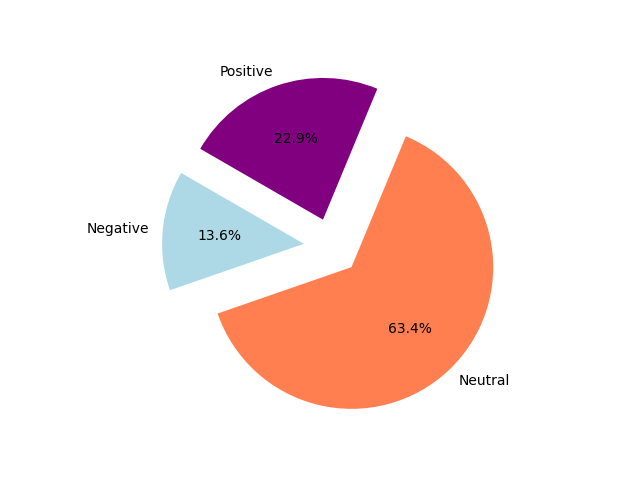
\includegraphics[height=3.5cm]{lisasVaderEmotionalPie.png}}
	{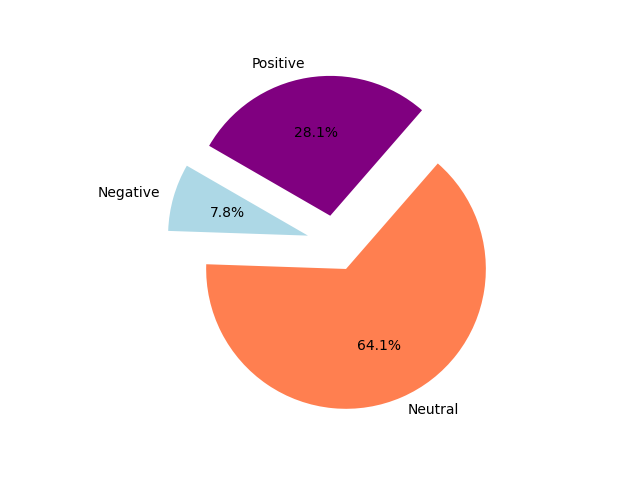
\includegraphics[height=3.5cm]{lisasBlobEmotionalPie.png}}
	{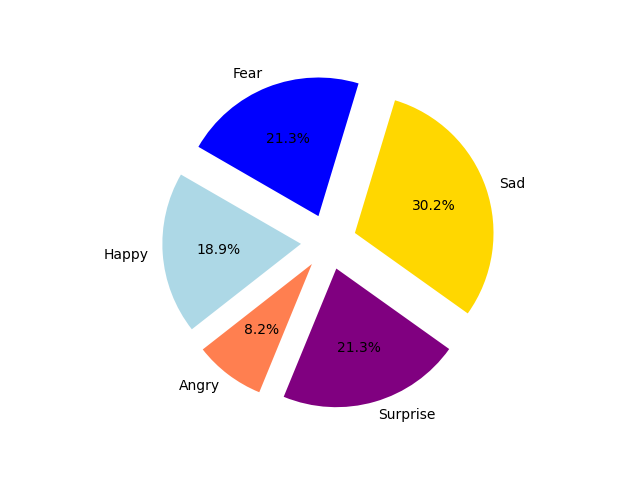
\includegraphics[height=3.5cm]{lisasEmotionalPie.png}}\\
	{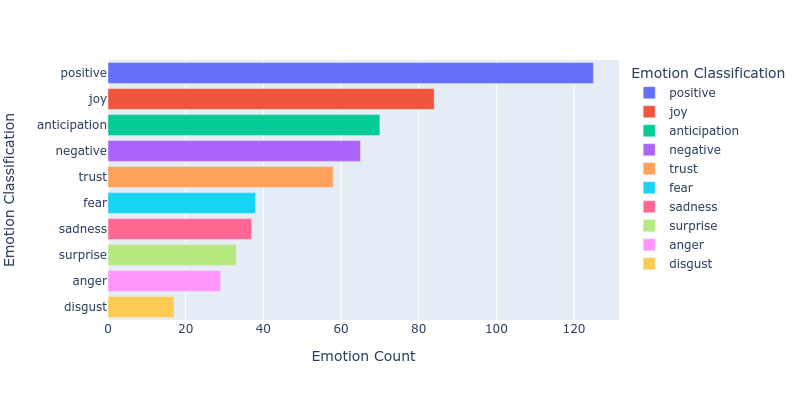
\includegraphics[width=17cm]{lisaNrcImage.png}}\\
	\clearpage
	\subsection{Johnny}
	{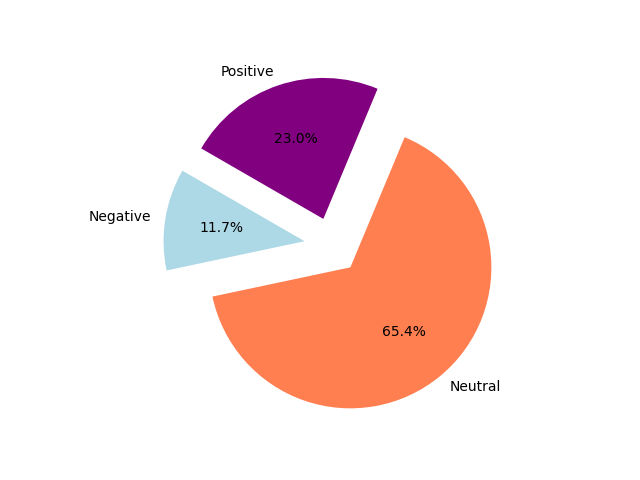
\includegraphics[height=3.5cm]{johnnysVaderEmotionalPie.png}}
	{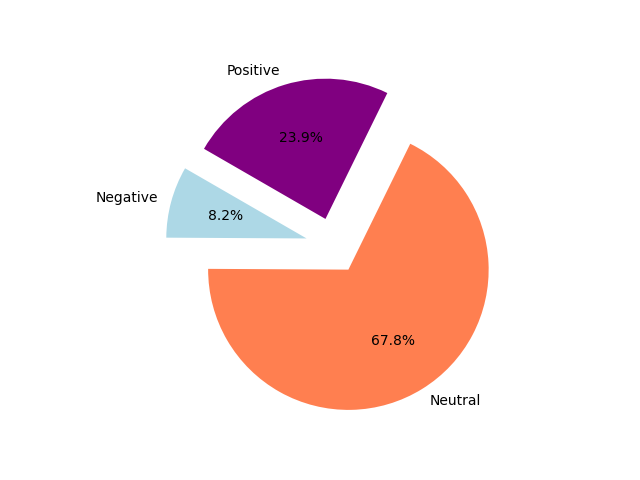
\includegraphics[height=3.5cm]{johnnysBlobEmotionalPie.png}}
	{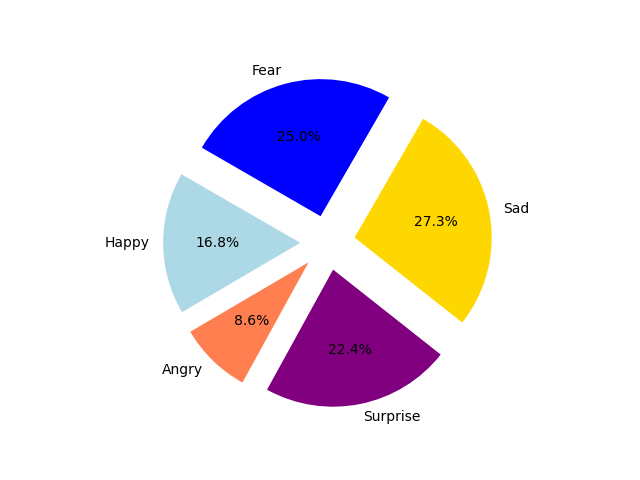
\includegraphics[height=3.5cm]{johnnysEmotionalPie.png}}\\
	{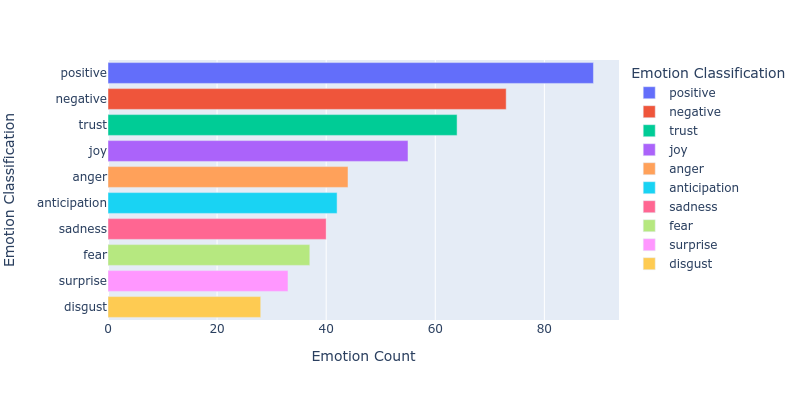
\includegraphics[width=17cm]{johnnyNrcImage.png}}\\
	\clearpage
	\subsection{Mark}
	{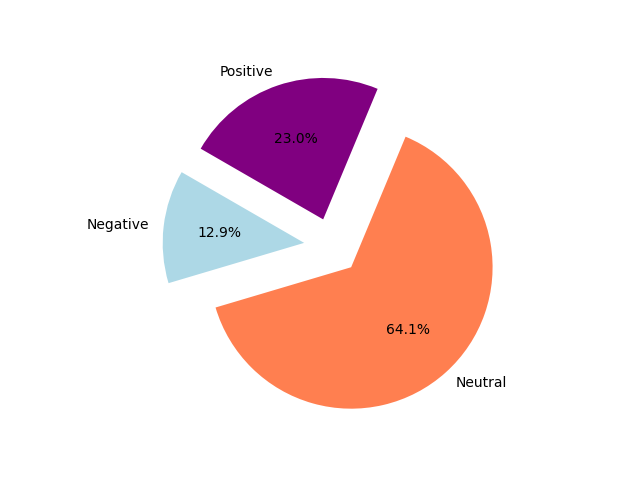
\includegraphics[height=3.5cm]{marksVaderEmotionalPie.png}}
	{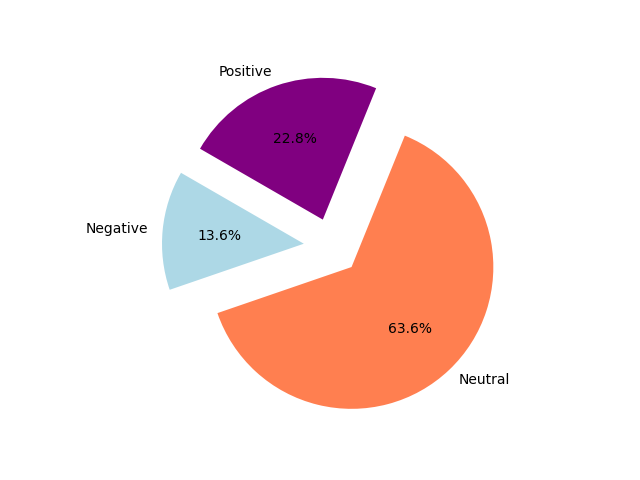
\includegraphics[height=3.5cm]{marksBlobEmotionalPie.png}}
	{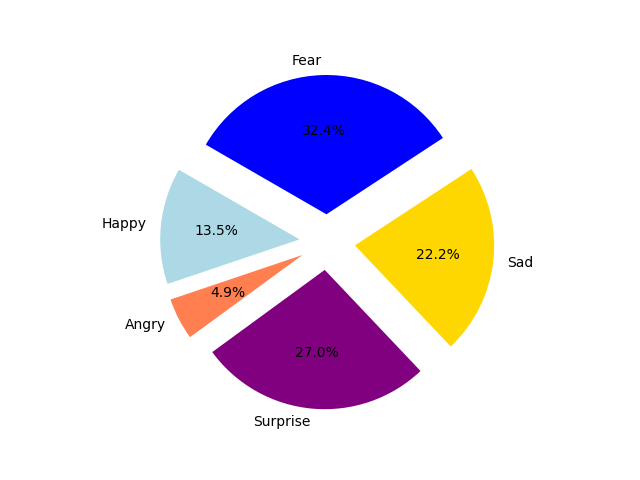
\includegraphics[height=3.5cm]{marksEmotionalPie.png}}\\
	{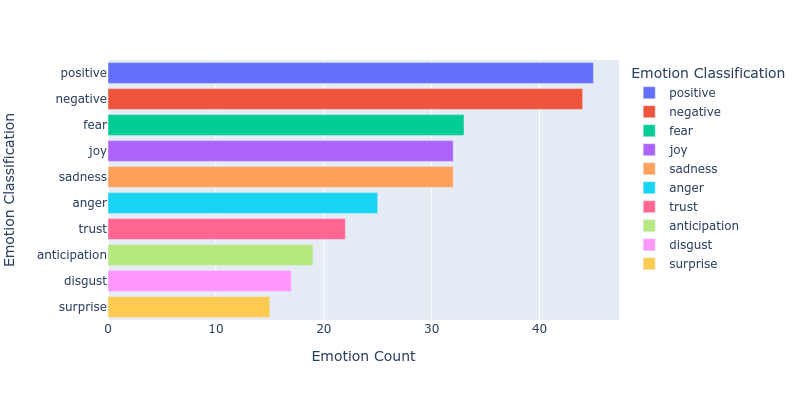
\includegraphics[width=17cm]{markNrcImage.png}}\\
	\clearpage
	\subsection{Claudette}
	{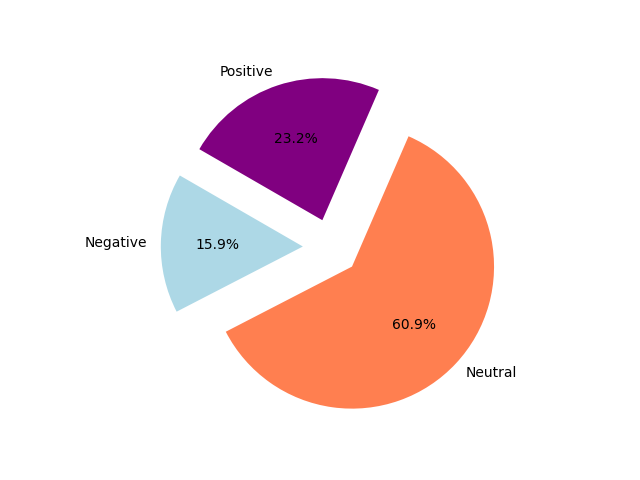
\includegraphics[height=3.5cm]{claudettesVaderEmotionalPie.png}}
	{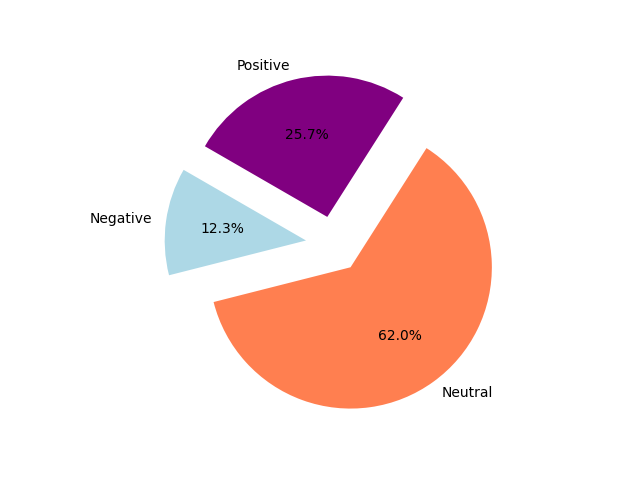
\includegraphics[height=3.5cm]{claudettesBlobEmotionalPie.png}}
	{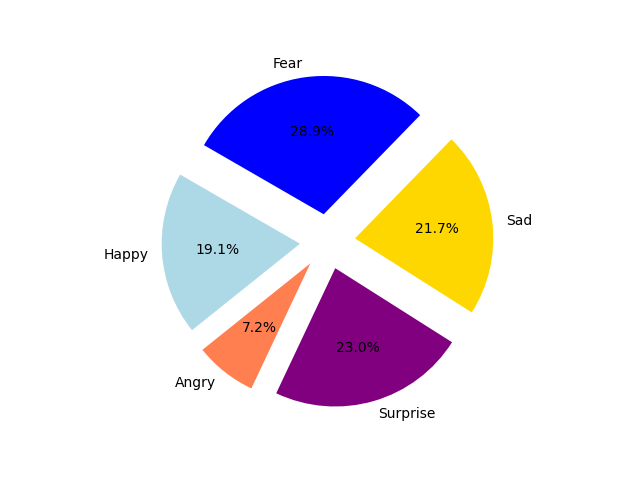
\includegraphics[height=3.5cm]{claudettesEmotionalPie.png}}\\
	{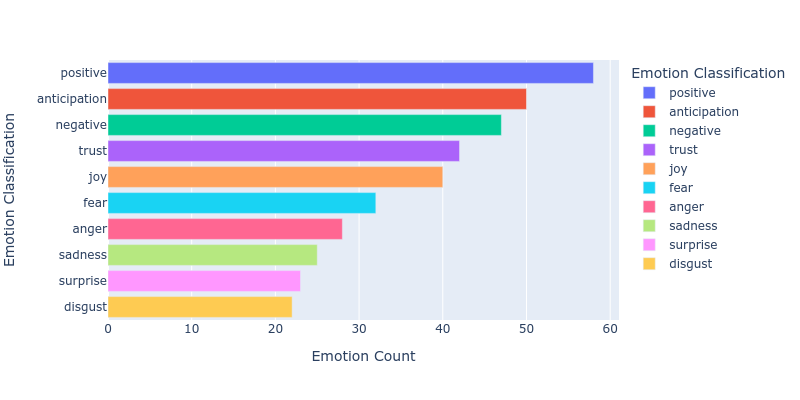
\includegraphics[width=17cm]{claudetteNrcImage.png}}\\
	\clearpage
	\subsection{Michelle}
	{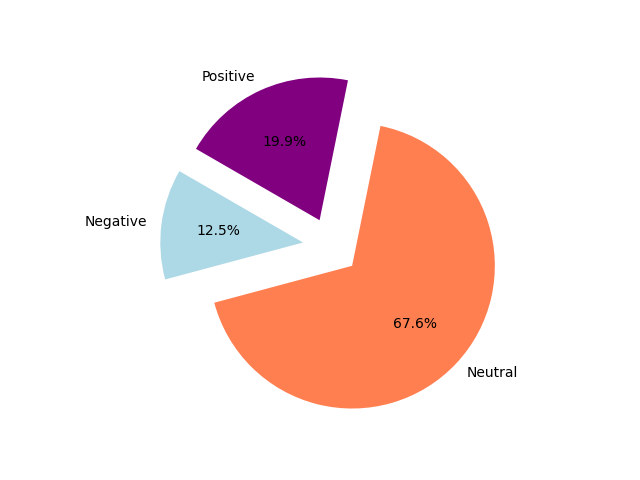
\includegraphics[height=3.5cm]{michellesVaderEmotionalPie.png}}
	{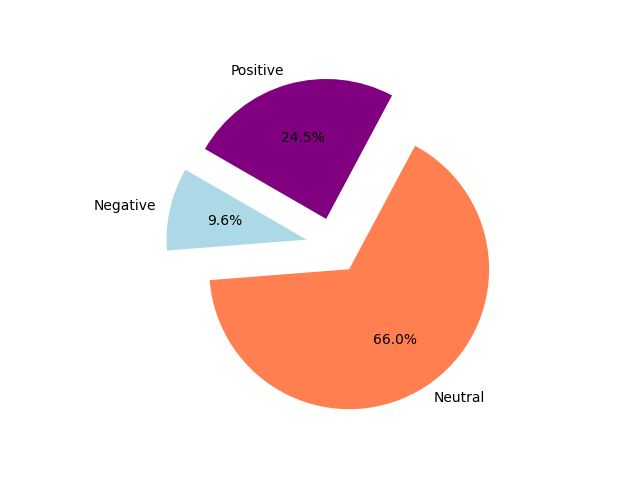
\includegraphics[height=3.5cm]{michellesBlobEmotionalPie.png}}
	{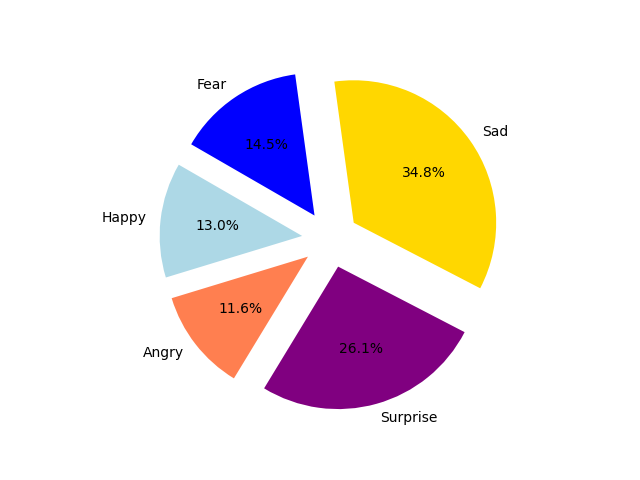
\includegraphics[height=3.5cm]{michellesEmotionalPie.png}}\\
	{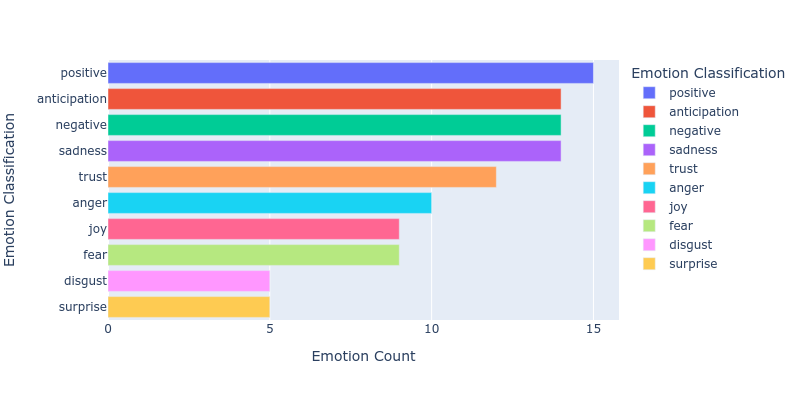
\includegraphics[width=17cm]{michelleNrcImage.png}}\\
	\clearpage
	\subsection{Peter}
	{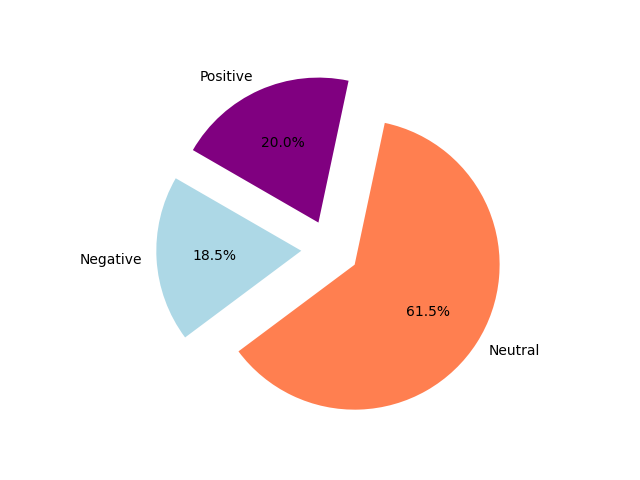
\includegraphics[height=3.5cm]{petersVaderEmotionalPie.png}}
	{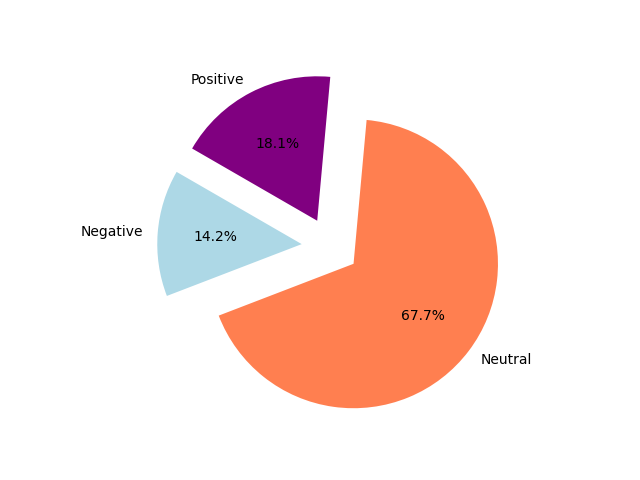
\includegraphics[height=3.5cm]{petersBlobEmotionalPie.png}}
	{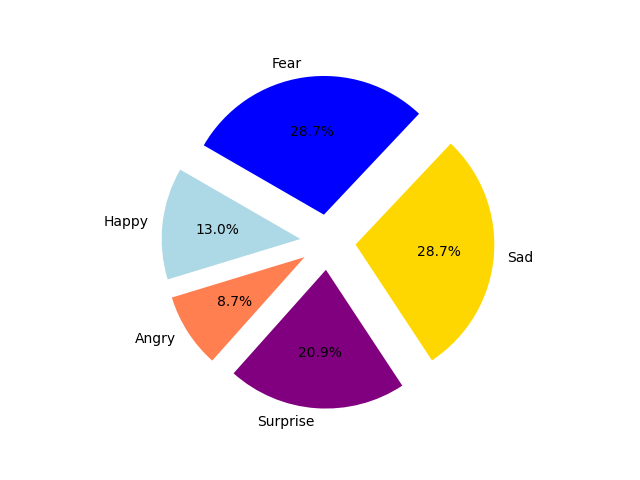
\includegraphics[height=3.5cm]{petersEmotionalPie.png}}\\
	{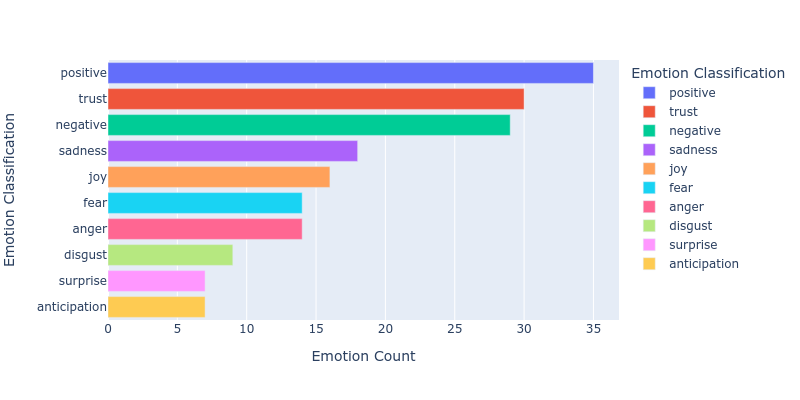
\includegraphics[width=17cm]{peterNrcImage.png}}\\
\end{document}